\batchmode
\makeatletter
\def\input@path{{/Users/quast/Thesis//}}
\makeatother
\documentclass[british]{article}\usepackage[]{graphicx}\usepackage[]{color}
%% maxwidth is the original width if it is less than linewidth
%% otherwise use linewidth (to make sure the graphics do not exceed the margin)
\makeatletter
\def\maxwidth{ %
  \ifdim\Gin@nat@width>\linewidth
    \linewidth
  \else
    \Gin@nat@width
  \fi
}
\makeatother

\definecolor{fgcolor}{rgb}{0.345, 0.345, 0.345}
\newcommand{\hlnum}[1]{\textcolor[rgb]{0.686,0.059,0.569}{#1}}%
\newcommand{\hlstr}[1]{\textcolor[rgb]{0.192,0.494,0.8}{#1}}%
\newcommand{\hlcom}[1]{\textcolor[rgb]{0.678,0.584,0.686}{\textit{#1}}}%
\newcommand{\hlopt}[1]{\textcolor[rgb]{0,0,0}{#1}}%
\newcommand{\hlstd}[1]{\textcolor[rgb]{0.345,0.345,0.345}{#1}}%
\newcommand{\hlkwa}[1]{\textcolor[rgb]{0.161,0.373,0.58}{\textbf{#1}}}%
\newcommand{\hlkwb}[1]{\textcolor[rgb]{0.69,0.353,0.396}{#1}}%
\newcommand{\hlkwc}[1]{\textcolor[rgb]{0.333,0.667,0.333}{#1}}%
\newcommand{\hlkwd}[1]{\textcolor[rgb]{0.737,0.353,0.396}{\textbf{#1}}}%

\usepackage{framed}
\makeatletter
\newenvironment{kframe}{%
 \def\at@end@of@kframe{}%
 \ifinner\ifhmode%
  \def\at@end@of@kframe{\end{minipage}}%
  \begin{minipage}{\columnwidth}%
 \fi\fi%
 \def\FrameCommand##1{\hskip\@totalleftmargin \hskip-\fboxsep
 \colorbox{shadecolor}{##1}\hskip-\fboxsep
     % There is no \\@totalrightmargin, so:
     \hskip-\linewidth \hskip-\@totalleftmargin \hskip\columnwidth}%
 \MakeFramed {\advance\hsize-\width
   \@totalleftmargin\z@ \linewidth\hsize
   \@setminipage}}%
 {\par\unskip\endMakeFramed%
 \at@end@of@kframe}
\makeatother

\definecolor{shadecolor}{rgb}{.97, .97, .97}
\definecolor{messagecolor}{rgb}{0, 0, 0}
\definecolor{warningcolor}{rgb}{1, 0, 1}
\definecolor{errorcolor}{rgb}{1, 0, 0}
\newenvironment{knitrout}{}{} % an empty environment to be redefined in TeX

\usepackage{alltt}
\usepackage[T1]{fontenc}
\usepackage[latin9]{inputenc}
\usepackage{babel}
\usepackage{float}
\usepackage[unicode=true,
 bookmarks=true,bookmarksnumbered=false,bookmarksopen=false,
 breaklinks=false,pdfborder={0 0 0},backref=false,colorlinks=false]
 {hyperref}
\hypersetup{
 pdfauthor={Bastiaan Quast}}

\makeatletter
%%%%%%%%%%%%%%%%%%%%%%%%%%%%%% Textclass specific LaTeX commands.
\newcommand{\code}[1]{\texttt{#1}}

%%%%%%%%%%%%%%%%%%%%%%%%%%%%%% User specified LaTeX commands.
\usepackage{appendix}
\usepackage[style=philosophy-modern,natbib=true,backend=biber]{biblatex}
\addbibresource{/Users/quast/Thesis/bibliography.bib}

\makeatother

\usepackage{listings}
\IfFileExists{upquote.sty}{\usepackage{upquote}}{}
\begin{document}

\title{\code{rnn}: a Recurrent Neural Network in R\thanks{https://cran.r-project.org/package=rnn | https://github.com/bquast/rnn}}


\author{Bastiaan Quast\thanks{http://qua.st | bastiaan.quast@graduateinstitute.ch | bquast@gmail.com}}

\maketitle
\vfill{}

\begin{abstract}
The rnn package implements a Recurrent Neural Network (RNN). RNN algorithms
have the ability to train neural networks to deal with greater levels
of complexity . This package is purposely designed to demonstrate
the self learning ability using the classic example of binary summation
on a bit-by-bit (right to left) basis, which requires the model to
develop the understanding that if a \code{1} and a \code{1} are
added, the outcome is \code{0}, but in the next iteration, it has
to that it was carrying a \code{1} from the previous iteration.
\end{abstract}
\newpage{}


\section{Introduction}

This package implements a Recurrent Neural Network which is trained
to sum 8-bit binary numbers, teaching itself the complex task of carrying
a 1 over to the next iteration if the sum of a column takes two bits
of space.

to convert numbers in range of 0-127 to binary representation.





Of course, numbers < 128 can be represent in a 7-bit binary form,
but since we are adding two numbers in the range 0-127, the total
can reach and achieve 128, which requires 8 bits, it cannot be more
than 254, the limit of 8 bit binary representation is 255, thereby
preventing overflows.

At this point it is useful to clarrify the nomenclature in this article.
I use the term RNN (capitalised) for the general concept of a Recurrent
Neural Network and I use \code{rnn} (in miniscules and using a monospace
font) to refer to the R package.



\begin{table}[H]
\caption{Package}


\begin{knitrout}
\definecolor{shadecolor}{rgb}{0.969, 0.969, 0.969}\color{fgcolor}\begin{kframe}
\begin{alltt}
\hlcom{# load the package}
\hlkwd{library}\hlstd{(rnn)}

\hlcom{# list functions}
\hlkwd{ls}\hlstd{(}\hlstr{'package:rnn'}\hlstd{)}
\end{alltt}
\begin{verbatim}
## [1] "bin2int"                      "int2bin"                     
## [3] "predictr"                     "sigmoid"                     
## [5] "sigmoid_output_to_derivative" "trainr"
\end{verbatim}
\end{kframe}
\end{knitrout}
\end{table}


As is listed above, the package contains the following functions:
\begin{itemize}
\item \code{bin2int()}: conversion of a matrix of numbers in binary representation
to decimal representation;
\item \code{int2bin()}: conversion of a vector numbers in decimal representation
to binary representation;
\item \code{predictr()}: predicts response variable based on a \code{trainr()}
model and input data;
\item \code{sigmoid()}: converts any number to a probability between 0
and 1;
\item \code{sigmoid\_output\_to\_derivative()}: takes output of \code{sigmoid()}
and gives point derivative;
\item \code{trainr()}: primary function, trains a model based on training
data and hyperparameters.
\end{itemize}
In addition to these functions there are also two internal functions
\code{i2b()} and \code{b2i()}, these functions are used by \code{int2bin()}
and \code{bin2int()} internally to change a single number from decimal
to binary or visa versa.


\section{Data}

The main \code{trainr()} function takes three integer vectors as
inputs: Y, X1, and X2. The vectors X1 and X2 are independent variables,
the Y vector is the sum of X1 and X2 and acts as the response variable
(for more info see \code{help('trainr')}).

Training data can be generated using base package's \code{sample()}
function. For reproducibility, we also set the seed value of the psuedo-random
number generator that \code{R} uses internally to \code{1}. After
generating \code{X1} and \code{X2}, I add the two pairwise and store
the result in \code{Y}. Finally, I convert both the input variables
and the response variable to binary representation using the \code{int2bin()}
included with the package.

\begin{table}[H]
\caption{Training Data}


\begin{knitrout}
\definecolor{shadecolor}{rgb}{0.969, 0.969, 0.969}\color{fgcolor}\begin{kframe}
\begin{alltt}
\hlcom{# use the same random numbers}
\hlkwd{set.seed}\hlstd{(}\hlnum{1}\hlstd{)}

\hlcom{# create training inputs }
\hlstd{X1} \hlkwb{=} \hlkwd{sample}\hlstd{(}\hlnum{0}\hlopt{:}\hlnum{127}\hlstd{,} \hlnum{7000}\hlstd{,} \hlkwc{replace}\hlstd{=}\hlnum{TRUE}\hlstd{)}
\hlstd{X2} \hlkwb{=} \hlkwd{sample}\hlstd{(}\hlnum{0}\hlopt{:}\hlnum{127}\hlstd{,} \hlnum{7000}\hlstd{,} \hlkwc{replace}\hlstd{=}\hlnum{TRUE}\hlstd{)}

\hlcom{# create training output }
\hlstd{Y} \hlkwb{<-} \hlstd{X1} \hlopt{+} \hlstd{X2}
\end{alltt}
\end{kframe}
\end{knitrout}
\end{table}


Internally the \code{int2bin()} function converts these characters
into binary format using the \code{intToBits()} function, the \code{bin2int()}
fucntion converts it back into decimal format for printing using the
\code{packBits()} function, both functions are included in the \code{base}
package.

We can for instance take the first value of \code{X1} and convert
it to a binary representation, whereby the \code{binary\_dim} argument
to the \code{trainr()} function determines the length of the binary
representation, throughout this paper we will use 8 bit representations
(which limits numbers to the range 0-255), but the theoretical limit
is 32 bits.

\begin{table}[H]


\caption{Binary Representation}


\begin{knitrout}
\definecolor{shadecolor}{rgb}{0.969, 0.969, 0.969}\color{fgcolor}\begin{kframe}
\begin{alltt}
\hlkwd{int2bin}\hlstd{( X1[}\hlnum{1}\hlstd{] )}
\end{alltt}
\begin{verbatim}
##      [,1] [,2] [,3] [,4] [,5] [,6] [,7] [,8]
## [1,]    0    0    1    0    0    0    0    1
\end{verbatim}
\end{kframe}
\end{knitrout}

\end{table}


Lets check look at the first sum in decimal representation.

\begin{table}[H]


\caption{Decimal Summation}


\begin{knitrout}
\definecolor{shadecolor}{rgb}{0.969, 0.969, 0.969}\color{fgcolor}\begin{kframe}
\begin{alltt}
\hlstd{X1[}\hlnum{1}\hlstd{]}
\end{alltt}
\begin{verbatim}
## [1] 33
\end{verbatim}
\begin{alltt}
\hlstd{X2[}\hlnum{1}\hlstd{]}
\end{alltt}
\begin{verbatim}
## [1] 89
\end{verbatim}
\begin{alltt}
\hlstd{X1[}\hlnum{1}\hlstd{]} \hlopt{+} \hlstd{X2[}\hlnum{1}\hlstd{]}
\end{alltt}
\begin{verbatim}
## [1] 122
\end{verbatim}
\begin{alltt}
\hlstd{Y[}\hlnum{1}\hlstd{]}
\end{alltt}
\begin{verbatim}
## [1] 122
\end{verbatim}
\end{kframe}
\end{knitrout}

\end{table}


and now in binary representation.

\begin{table}[H]


\caption{Binary Summation}


\begin{knitrout}
\definecolor{shadecolor}{rgb}{0.969, 0.969, 0.969}\color{fgcolor}\begin{kframe}
\begin{alltt}
\hlkwd{int2bin}\hlstd{( X1[}\hlnum{1}\hlstd{] )}
\hlkwd{int2bin}\hlstd{( X2[}\hlnum{1}\hlstd{] )}
\hlkwd{print}\hlstd{(}\hlstr{'--------------------------------------'}\hlstd{)}
\hlkwd{int2bin}\hlstd{( Y[}\hlnum{1}\hlstd{]  )}
\end{alltt}
\begin{verbatim}
##      [,1] [,2] [,3] [,4] [,5] [,6] [,7] [,8]
## [1,]    0    0    1    0    0    0    0    1
##      [,1] [,2] [,3] [,4] [,5] [,6] [,7] [,8]
## [1,]    0    1    0    1    1    0    0    1
## [1] "--------------------------------------"
##      [,1] [,2] [,3] [,4] [,5] [,6] [,7] [,8]
## [1,]    0    1    1    1    1    0    1    0
\end{verbatim}
\end{kframe}
\end{knitrout}

\end{table}


As can be seen from the above output, the first values of \code{X1}
and \code{X2}, \code{33} and \code{89} respectively, are both in
the range 0-127, which can be represented with only 7 bits. Yet the
sum of the two - 122 - is almost outside of the range 0-127, which
is why an 8th bit is required (i.e. the 8th value from right to left
in the bottom row is \code{1}). If we sampled numbers great than
127 for \code{X1} and \code{X2} then the sum of the two could be
greater than 255, which requires a ninth bit (or \code{length=9}).

We can now convert the entire vectors to binary matrices.

\begin{knitrout}
\definecolor{shadecolor}{rgb}{0.969, 0.969, 0.969}\color{fgcolor}\begin{kframe}
\begin{alltt}
\hlcom{# convert to binaries of 8 bit (default)}
\hlstd{X1} \hlkwb{<-} \hlkwd{int2bin}\hlstd{(X1)}
\hlstd{X2} \hlkwb{<-} \hlkwd{int2bin}\hlstd{(X2)}
\hlstd{Y}  \hlkwb{<-} \hlkwd{int2bin}\hlstd{(Y)}
\end{alltt}
\end{kframe}
\end{knitrout}

The rnn() function will run until it has evaluated all values in the
vector that it is fed. Since the training of the network, particularly
the carrying part, takes many iterations to learn (the exact number
of iterations varies but depends on the hyperparameters, more on this
in the next section), it is therefore advisable to sample several
thousand values (I use 7000).


\section{Methodology}

The workhorse of the \code{rnn} package is the \code{trainr()} function.

For example, if we add the binary numbers \code{0 0 1} (decimal system:
1) and \code{1 0 1} (decimal system: 5), we start by adding the right
column, \code{1} and \code{1} make \code{1 0} (similar to when
5 and 5 make 1 0 in the decimal system) , the \code{0} is stored
in the right column, the \code{1} is carried over to the middle column
and added with the two existing bits \code{0} and \code{0}, to form
\code{1}, which is stored in the middle column. This time nothing
is carried over and the left column sums \code{0} and \code{1} to
make \code{1}, which gives the outcome \code{1 1 0} (decimal system:
6).

If we go back to the output of the int2binary() function for X1, X2,
and Y, we see that in the 4th column (from right to left), a 0 and
a 0 are added, resulting in an output of 1. This is because in the
previous iteration 3rd column (from right to left) a 1 and a 1 are
added, which becomes 1 0, so the 0 goes in column 3 and the 1 is carried
over to colum 4. Since the summation is done bit by bit (or column
by column), the neural network need to remember from the 3rd iteration
until the 4th interation that it is carrying a 1 over. It is this
remembering that a feed-forward neural network cannot teach itself.

The rnn() function internally makes use of the \code{sigmoid()} function,
which is a very simple implementation of a sigmoid which takes the
range (-Infinity, Infinity) and maps it to the range (0, 1).

\begin{table}[H]


\caption{Sigmoid Source Code}


\begin{knitrout}
\definecolor{shadecolor}{rgb}{0.969, 0.969, 0.969}\color{fgcolor}\begin{kframe}
\begin{alltt}
\hlcom{# print source code of the sigmoid function}
\hlstd{sigmoid}
\end{alltt}
\begin{verbatim}
## function(x) {
##   output = 1 / (1+exp(-x))
##   return(output)            }
## <environment: namespace:rnn>
\end{verbatim}
\end{kframe}
\end{knitrout}

\end{table}


For instance:

\begin{table}[H]


\caption{Sigmoid Examples}


\begin{knitrout}
\definecolor{shadecolor}{rgb}{0.969, 0.969, 0.969}\color{fgcolor}\begin{kframe}
\begin{alltt}
\hlkwd{sigmoid}\hlstd{(}\hlopt{-}\hlnum{137}\hlstd{)}
\hlkwd{sigmoid}\hlstd{(}\hlnum{5.3}\hlstd{)}
\end{alltt}
\begin{verbatim}
## [1] 3.174359e-60
## [1] 0.9950332
\end{verbatim}
\end{kframe}
\end{knitrout}

\end{table}


The shape of the sigmoid function is as follows.

\begin{figure}[H]


\caption{Sigmoid Shape}


\begin{knitrout}
\definecolor{shadecolor}{rgb}{0.969, 0.969, 0.969}\color{fgcolor}\begin{kframe}
\begin{alltt}
\hlkwd{library}\hlstd{(ggplot2)} \hlcom{# load plotting package}

\hlcom{# plot sigmoid shape}
\hlkwd{qplot}\hlstd{(}\hlkwd{seq}\hlstd{(}\hlopt{-}\hlnum{10}\hlopt{:}\hlnum{10}\hlstd{),} \hlkwd{sigmoid}\hlstd{(}\hlkwd{seq}\hlstd{(}\hlopt{-}\hlnum{10}\hlstd{,}\hlnum{10}\hlstd{)),} \hlkwc{geom}\hlstd{=}\hlstr{'line'}\hlstd{)}
\end{alltt}
\end{kframe}
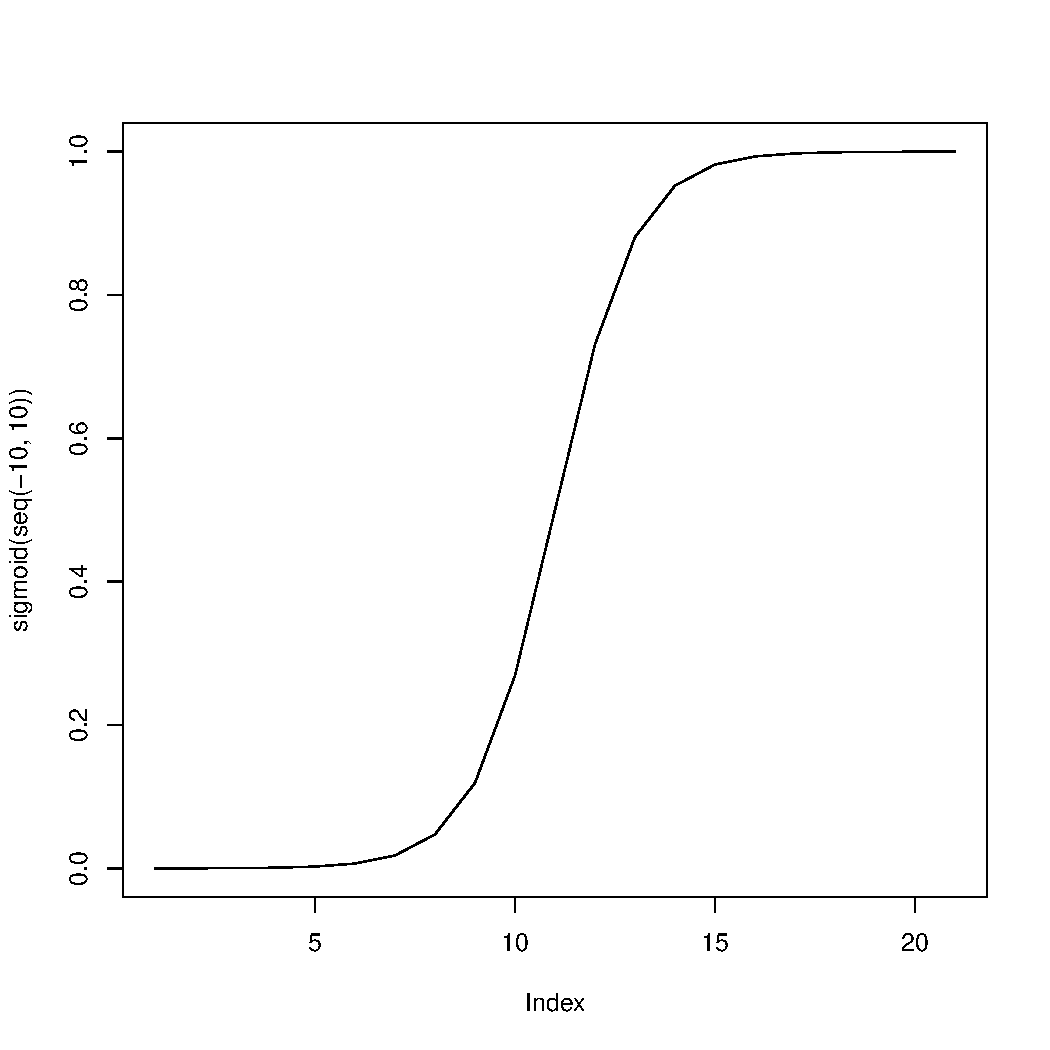
\includegraphics[width=\maxwidth]{figure/sigmoid_shape-1} 

\end{knitrout}

\end{figure}


Additionally the rnn() function uses the sigmoid\_output\_to\_derivative()
function.

\begin{table}[H]


\caption{Sigmoid Derivative Source Code}


\begin{knitrout}
\definecolor{shadecolor}{rgb}{0.969, 0.969, 0.969}\color{fgcolor}\begin{kframe}
\begin{alltt}
\hlcom{# print source code of the sigmoid_output_to_derivate function}
\hlstd{sigmoid_output_to_derivative}
\end{alltt}
\begin{verbatim}
## function(output) {
##   return( output*(1-output) )                      }
## <environment: namespace:rnn>
\end{verbatim}
\end{kframe}
\end{knitrout}

\end{table}


As the purpose of the package is to illustrate the working of a Recurrent
Neural Network, the \code{trainr()} function is quite verbose (this
can be controlled using the \code{print} argument).

\begin{table}[H]


\caption{trainr() Output}


\begin{knitrout}\tiny
\definecolor{shadecolor}{rgb}{0.969, 0.969, 0.969}\color{fgcolor}\begin{kframe}
\begin{verbatim}
## [1] "Summation number: 1000"
## [1] "x1: 1"
## [1] "x2: 1 +"
## [1] "-------"
## [1] "y:  0"
## [1] "y^: 1"
## [1] "======="
## [1] "x1: 0"
## [1] "x2: 0 +"
## [1] "-------"
## [1] "y:  1"
## [1] "y^: 1"
## [1] "======="
## [1] "x1: 0"
## [1] "x2: 0 +"
## [1] "-------"
## [1] "y:  0"
## [1] "y^: 0"
## [1] "======="
## [1] "x1: 0"
## [1] "x2: 0 +"
## [1] "-------"
## [1] "y:  0"
## [1] "y^: 0"
## [1] "======="
## [1] "x1: 0"
## [1] "x2: 1 +"
## [1] "-------"
## [1] "y:  1"
## [1] "y^: 0"
## [1] "======="
## [1] "x1: 1"
## [1] "x2: 1 +"
## [1] "-------"
## [1] "y:  0"
## [1] "y^: 1"
## [1] "======="
## [1] "x1: 0"
## [1] "x2: 0 +"
## [1] "-------"
## [1] "y:  1"
## [1] "y^: 1"
## [1] "======="
## [1] "x1: 0"
## [1] "x2: 0 +"
## [1] "-------"
## [1] "y:  0"
## [1] "y^: 0"
## [1] "======="
## [1] "Error: 3.87983649375435"
## [1] "X1[ 1000 ]: 0 0 1 0 0 0 0 1   ( 33 )"
## [1] "X2[ 1000 ]: 0 0 1 1 0 0 0 1 + ( 49 )"
## [1] "-----------------------------"
## [1] "Y[ 1000 ]:  0 1 0 1 0 0 1 0   ( 82 )"
## [1] "predict Y^: 0 1 1 0 0 0 1 1   ( 99 )"
## [1] "============================="
\end{verbatim}
\end{kframe}
\end{knitrout}

\end{table}


The text printed here is of the 8 steps of the summation of the 1000th
value of \code{X1} and \code{X2}, or iteration 7993-8000.

Each iteration is printed individually, with the two input bits, the
prediction for the response value and the actual response value.

After each iternation the difference betweeen the predicted value
and the actual value is fed back into the neural network using a method
called back-propagation (an application the chain rule of differential
calculus).

At the end of the 8 iterations that it here takes to add two values
of \code{X1} and \code{X2}, the results are printed in a more human
legible form. It should be clear from the results that after 1000
numbers, which 8 iterations each, the model is still performing very
poorly.

However, progress can be observed:

\begin{table}[H]
\caption{trainr() Output}


\begin{knitrout}\tiny
\definecolor{shadecolor}{rgb}{0.969, 0.969, 0.969}\color{fgcolor}\begin{kframe}
\begin{alltt}
\hlcom{# use the same random numbers}
\hlkwd{set.seed}\hlstd{(}\hlnum{1}\hlstd{)}

\hlcom{# train the network}
\hlstd{m1} \hlkwb{<-} \hlkwd{trainr}\hlstd{(Y,}
             \hlstd{X1,}
             \hlstd{X2,}
             \hlkwc{binary_dim} \hlstd{=}  \hlnum{8}\hlstd{,}
             \hlkwc{alpha}      \hlstd{=}  \hlnum{0.1}\hlstd{,}
             \hlkwc{input_dim}  \hlstd{=}  \hlnum{2}\hlstd{,}
             \hlkwc{hidden_dim} \hlstd{=} \hlnum{10}\hlstd{,}
             \hlkwc{output_dim} \hlstd{=}  \hlnum{1}\hlstd{,}
             \hlkwc{print} \hlstd{=} \hlstr{'minimal'} \hlstd{)}
\end{alltt}
\begin{verbatim}
## [1] "Summation number: 1000"
## [1] "Error: 3.90950698309064"
## [1] "X1[ 1000 ]: 0 0 0 0 1 1 0 1   ( 13 )"
## [1] "X2[ 1000 ]: 0 0 1 0 1 1 1 1 + ( 47 )"
## [1] "-----------------------------"
## [1] "Y[ 1000 ]:  0 0 1 1 1 1 0 0   ( 60 )"
## [1] "predict Y^: 0 1 1 1 1 1 1 1   ( 127 )"
## [1] "============================="
## [1] "Summation number: 2000"
## [1] "Error: 4.03678792609062"
## [1] "X1[ 2000 ]: 0 0 1 1 1 0 0 1   ( 57 )"
## [1] "X2[ 2000 ]: 0 1 1 0 0 1 0 0 + ( 100 )"
## [1] "-----------------------------"
## [1] "Y[ 2000 ]:  1 0 0 1 1 1 0 1   ( 157 )"
## [1] "predict Y^: 1 1 1 1 1 1 1 1   ( 255 )"
## [1] "============================="
## [1] "Summation number: 3000"
## [1] "Error: 4.0117145610462"
## [1] "X1[ 3000 ]: 0 1 0 1 0 1 1 1   ( 87 )"
## [1] "X2[ 3000 ]: 0 1 1 1 0 0 1 1 + ( 115 )"
## [1] "-----------------------------"
## [1] "Y[ 3000 ]:  1 1 0 0 1 0 1 0   ( 202 )"
## [1] "predict Y^: 1 0 0 0 0 1 0 0   ( 132 )"
## [1] "============================="
## [1] "Summation number: 4000"
## [1] "Error: 3.4363646618886"
## [1] "X1[ 4000 ]: 0 0 1 1 0 1 1 0   ( 54 )"
## [1] "X2[ 4000 ]: 0 0 1 1 1 0 0 0 + ( 56 )"
## [1] "-----------------------------"
## [1] "Y[ 4000 ]:  0 1 1 0 1 1 1 0   ( 110 )"
## [1] "predict Y^: 0 1 0 0 0 0 1 0   ( 66 )"
## [1] "============================="
## [1] "Summation number: 5000"
## [1] "Error: 2.26331897903431"
## [1] "X1[ 5000 ]: 0 0 0 0 0 0 0 1   ( 1 )"
## [1] "X2[ 5000 ]: 0 0 1 1 1 0 1 0 + ( 58 )"
## [1] "-----------------------------"
## [1] "Y[ 5000 ]:  0 0 1 1 1 0 1 1   ( 59 )"
## [1] "predict Y^: 0 0 1 1 1 1 0 1   ( 61 )"
## [1] "============================="
## [1] "Summation number: 6000"
## [1] "Error: 1.90553916946373"
## [1] "X1[ 6000 ]: 0 1 1 1 0 0 1 1   ( 115 )"
## [1] "X2[ 6000 ]: 0 0 1 0 0 1 0 1 + ( 37 )"
## [1] "-----------------------------"
## [1] "Y[ 6000 ]:  1 0 0 1 1 0 0 0   ( 152 )"
## [1] "predict Y^: 1 0 0 1 1 0 0 0   ( 152 )"
## [1] "============================="
## [1] "Summation number: 7000"
## [1] "Error: 0.992546604462261"
## [1] "X1[ 7000 ]: 0 1 0 1 0 1 1 1   ( 87 )"
## [1] "X2[ 7000 ]: 0 0 1 1 1 0 1 1 + ( 59 )"
## [1] "-----------------------------"
## [1] "Y[ 7000 ]:  1 0 0 1 0 0 1 0   ( 146 )"
## [1] "predict Y^: 1 0 0 1 0 0 1 0   ( 146 )"
## [1] "============================="
\end{verbatim}
\end{kframe}
\end{knitrout}

\end{table}


In fact, from the 6000th summation on, all the printed estimates are
in fact correct.


\section{Results}

The eventual purpose is to use the model generated by the \code{trainr()}
function as an input to the \code{predictr()} function, in order
to predict the values of new inputs.

\begin{table}[H]


\caption{Test Data}


\begin{knitrout}
\definecolor{shadecolor}{rgb}{0.969, 0.969, 0.969}\color{fgcolor}\begin{kframe}
\begin{alltt}
\hlcom{# create test inputs}
\hlstd{C1} \hlkwb{=} \hlkwd{int2bin}\hlstd{(} \hlkwd{sample}\hlstd{(}\hlnum{0}\hlopt{:}\hlnum{127}\hlstd{,} \hlnum{7000}\hlstd{,} \hlkwc{replace}\hlstd{=}\hlnum{TRUE}\hlstd{) )}
\hlstd{C2} \hlkwb{=} \hlkwd{int2bin}\hlstd{(} \hlkwd{sample}\hlstd{(}\hlnum{0}\hlopt{:}\hlnum{127}\hlstd{,} \hlnum{7000}\hlstd{,} \hlkwc{replace}\hlstd{=}\hlnum{TRUE}\hlstd{) )}
\end{alltt}
\end{kframe}
\end{knitrout}

\end{table}


Now predict using the \code{predictr() }function.

\begin{table}[H]


\caption{predictr()}


\begin{knitrout}
\definecolor{shadecolor}{rgb}{0.969, 0.969, 0.969}\color{fgcolor}\begin{kframe}
\begin{alltt}
\hlcom{# predic}
\hlstd{D}  \hlkwb{<-} \hlkwd{predictr}\hlstd{(m1,}
               \hlstd{C1,}
               \hlstd{C2,}
               \hlkwc{binary_dim} \hlstd{=}  \hlnum{8}\hlstd{,}
               \hlkwc{alpha}      \hlstd{=}  \hlnum{0.1}\hlstd{,}
               \hlkwc{input_dim}  \hlstd{=}  \hlnum{2}\hlstd{,}
               \hlkwc{hidden_dim} \hlstd{=} \hlnum{10}\hlstd{,}
               \hlkwc{output_dim} \hlstd{=}  \hlnum{1}   \hlstd{)}

\hlcom{# convert back to decimal}
\hlstd{C1} \hlkwb{<-} \hlkwd{bin2int}\hlstd{(C1)}
\hlstd{C2} \hlkwb{<-} \hlkwd{bin2int}\hlstd{(C2)}
\hlstd{D}  \hlkwb{<-} \hlkwd{bin2int}\hlstd{(D)}

\hlcom{# inspect the differences               }
\hlkwd{qplot}\hlstd{( D}\hlopt{-}\hlstd{(C1}\hlopt{+}\hlstd{C2) )}
\end{alltt}


{\ttfamily\noindent\itshape\color{messagecolor}{\#\# `stat\_bin()` using `bins = 30`. Pick better value with `binwidth`.}}\end{kframe}
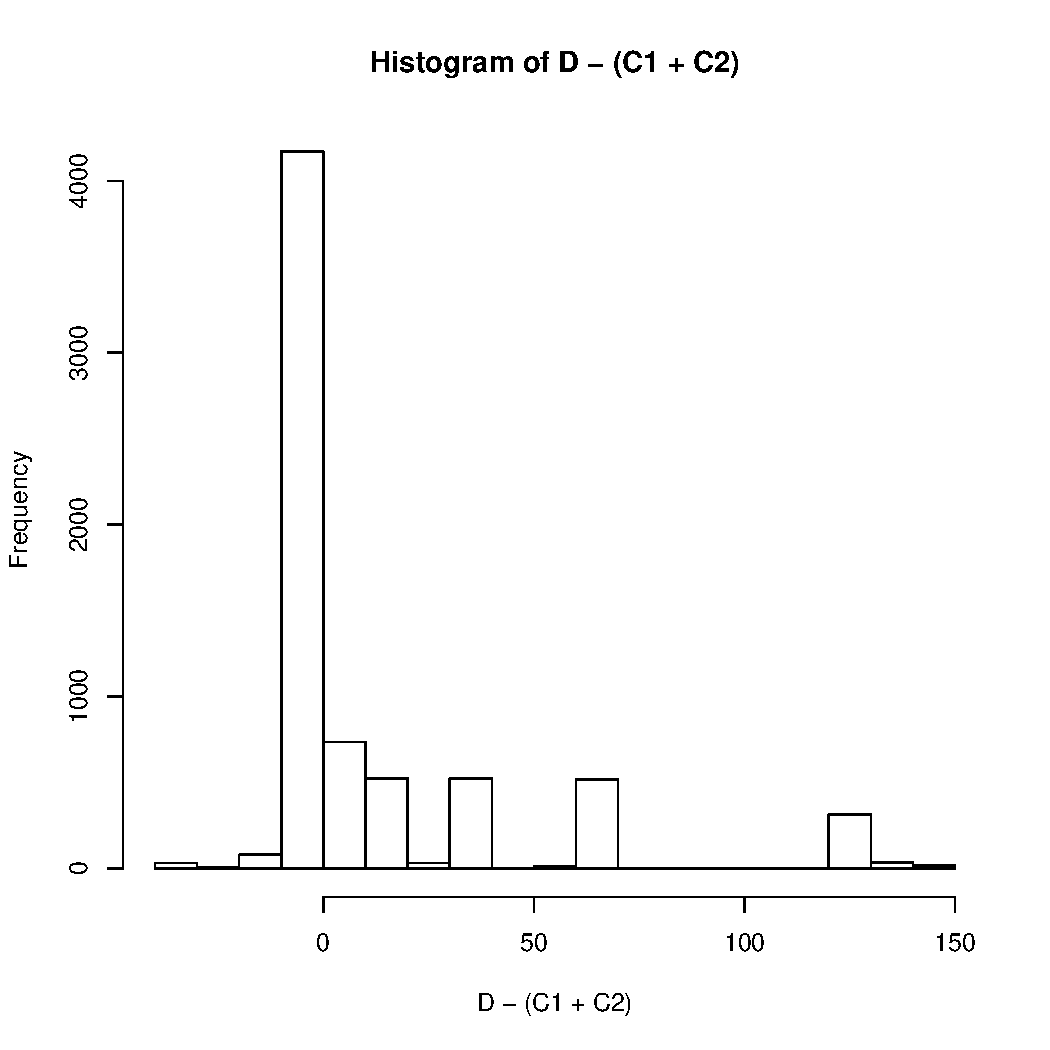
\includegraphics[width=\maxwidth]{figure/predictr-1} 

\end{knitrout}

\end{table}



\section{Conclusion}

CRAN and the rest of the R ecosystem show that there is a strong interest
in using the R language for neural network analysis. Existing package
such as the built in nnet package and the caret package make available
very powerful neural network tools to R users. The RSNNS package acts
as an R wrapper for the Stutgard Neural Network Simulator library,
which is written in C, and thereby makes available to partial RNNs
such as Elman and Jordan networks.

The enormous popularity of full Recurrent Neural Networks in other
languages, primarily Python and C, show that there is a great amount
of interest for using this methodology, including interest from Economist,
Data Scientists, and other non-professional programmers. Although
Python is a relatively accessible programming language for laymen,
it has a smaller user base in terms of data analists. The \code{rnn}
package attempts to address this need by showing that Recurrent Neural
Networks can be made available and perhaps more importantly, made
available in native R, which allows user to delve into the code and
understand the method and developer a more thorough understanding
of how to use it.

\pagebreak{}

\appendix

\section{Source code of \protect\code{trainr()} function}

\lstinputlisting[language=S,basicstyle={\footnotesize},numbers=left,numberstyle={\tiny},frame=single,breaklines=true,title={\lstname}]{0_Users_quast_rnn_R_trainr.R}


\section{Source code of \protect\code{predictr() }function}

\lstinputlisting[language=S,basicstyle={\footnotesize},numbers=left,numberstyle={\tiny},frame=single,breaklines=true,title={\lstname}]{1_Users_quast_rnn_R_predictr.R}
\end{document}
